\documentclass[letterpaper, 10 pt, conference]{ieeeconf}
\IEEEoverridecommandlockouts
\overrideIEEEmargins
\usepackage{cite}
\usepackage{algorithm}
\usepackage{algpseudocode}
\usepackage{amsmath}
\usepackage{amssymb}
\usepackage{graphics}
\usepackage{graphicx}
\usepackage{multirow}
\usepackage{rotating}
\usepackage{verbatim}
\usepackage[caption=false,font=footnotesize,subrefformat=parens,labelformat=parens]{subfig}
\graphicspath{{graphics/}}
\DeclareGraphicsExtensions{.png}
\title{\bf
Air-Hockey Robot
}

\author{\parbox{5 in}{\centering Daniel Koniar, Matthew Russell, and Steve Thomas}\\
  {\tt\small \{konia013, russe546, thom5159\}@umn.edu}\\
  Department of Computer Science and Engineering\\
  University of Minnesota\\
  Minneapolis, MN 55455\\
}  

\begin{document}
\maketitle
\thispagestyle{empty}
\pagestyle{empty}

%%%%%%%%%%%%%%%%%%%%%%%%%%%%%%%%%%%%%%%%%%%%%%%%%%%%%%%%%%%%%%%%%%%%%%%%%%%%%%%%
\begin{abstract}
This paper is a report detailing the progression of the plan to build and program a robot that is capable of playing Air Hockey.  The sections outlined in this paper are introduction, problem description, motivation, related work, and timeline.  The air hockey robot will built through the use of computer vision, robotic mechanisms, and artificial intelligence. The robotic manipulator is to be constructed using servo motors, which will allow for movement in a two-dimensional plane.  The computer vision portion will consist of a camera with a top-down view on the workspace.  This project will emphasize the combination of a robotic manipulator and computer vision in a fast-paced environment, which necessitates multiple metrics in order to attempt to reach a state of optimality.  On top of discussing and evaluating the construction of an Air-Hockey Robot, this paper will also display and discuss these metrics, which will be obtained through experimentation.  These metrics will be mentioned further in the following section.
\end{abstract}

%%%%%%%%%%%%%%%%%%%%%%%%%%%%%%%%%%%%%%%%%%%%%%%%%%%%%%%%%%%%%%%%%%%%%%%%%%%%%%%%
\section{Introduction}
\label{introduction}
Improvement in both robotic mechanisms and computer vision has allowed for the production of reactionary robots based in interpretation of surroundings.  The combination of these fields allow for a variety of specialized robotics, varying from robotic drones \cite{3dr} with ground recognition to self-driving cars \cite{googlecar}.  Artificial Intelligence  typically acts as some mediary layer between the robotic and computer vision layers.  Artificial intelligence allows for a goal to defined, or task, and the means of accomplishing reaching that goal.  It allows for reactionary response from the robotic mechanism in a changing environment through computational analysis.  One example of this would be automated assembly systems, where computer-vision object-recognition is used in order to have robotic manipulator to grasp and transport said object.

This project uses the combination of computer vision, robotic mechanisms, and artificial intelligence an order to create a  robot that is capable of playing Air Hockey. The artificial intelligence will be the key transitional level involved in the interpretation of computer vision images and computing the inputs for the appropriate reactionary movements of the robotic manipulator.  It will provide the necessary computations that will both link the computer vision layer to the robotic manipulator layer and produce a possibility for varying difficulties.  The computer vision part of our project will introduce the sensory component to our system and the robotic mechanism is the response component.

In this project, multiple aspects will be examined and discussed.  One aspect will be the analysis of the actual development and construction of the Air Hockey robot.  Once the robot is in full working operation, the experimental data will be gathered and examined, the metrics of which will be defined in the next paragraph.  If time permitting, some variance will be implemented into this system for further experimental examination and comparison.  The last aspect of the project that will be examined is the entirety of project in a retrospective lens.  The analysis of this will include what could be done to make the system better and what failures were experienced.

There are many key metrics for the Air-Hockey Robot an order to attempt to reach an optimal state. The metrics that will be mainly emphasized are efficiency, reactionary time, accuracy, and repeatability. To further define these, efficiency will be defined as minimizing the movements necessary to be made by the robotic manipulator an order to hit the puck.  Reactionary time will be defined as the amount of time needed to go from raw images to movement input to the robotic manipulator. Accuracy will be defined as how often the puck can be reached and hit in the desired direction [with a small error tolerance].  Repeatability will be defined as the robotic manipulator’s ability to repeat an action precisely, provided the exact same environment/situation. For instance, if a puck were sent from the same exact direction and with the exact velocity one hundred times, repeatability would be the number instances where the robotic manipulator could hit the puck in the same exact way.

%%%%%%%%%%%%%%%%%%%%%%%%%%%%%%%%%%%%%%%%%%%%%%%%%%%%%%%%%%%%%%%%%%%%%%%%%%%%%%%%
\section{Problem Description}
\label{sec:problem_description}
\subsection{Definition of Problem}
With recent advances in computer processing and affordability, computers and robotics are increasingly used for recreational tasks.  The possibility of constructing a robotic system to play Air Hockey, a simple two-dimensional game in real space, will be explored in this project. By combining computer vision, robotic mechanisms, and A.I. algorithms, a Hockey playing robot can be implemented with a goal-oriented approach to allow the robotic system to react to a human opponent’s actions and quickly derive a solution. The setup will require an overhead camera which monitors the puck movement and robotic manipulator with the end effector being the opponent player. The manipulator will be ported onto the workspace, being the air hockey field, and will be interfaced through a computer (Raspberry Pi 2). 

The camera will track the puck movement in a two dimensional plane and the data will be processed through the computer vision software to compute the trajectory of the puck.  The trajectory will then be used by the mediary software to predict the movements for the robotic manipulator an order to strike the puck back towards the opposite goal [from which the robotic manipulator is defending].  The mediary software will handle the transition of data from the computer vision to the robotic manipulator as well as the artificial intelligence schema (which will most likely be a path-finding algorithm with a heuristic) which will compute how the manipulator should react. The end effector will thus be controlled through a combination of robotic mechanisms and artificial intelligence in a reactionary setting.
\subsection{Motivation}
Computer Vision is widely used today with its applications ranging from traffic control\cite{aliane} to gesture recognition \cite{bhame}. Our primary motivation is to grasp an understanding of how we use computer vision. Computer Vision is a tool used in robotics to process and understand images from the real word.The robotic system takes in this image data and performs selective tasks based on the algorithms and functions written within the system. Our secondary motivation is to learn how we interface between the the two different categorical hardware and combining them through a software layer. This will enable us develop skills in building and programming robots which is the resultant goal this project. Finally, we also desire to increase understanding about the  significance of robotic precision. Since the system response needs to be almost instantaneous, the robotic hardware needs to be efficient, quick and accurate with minimal margin for error. This falls back on the metric of Accuracy, which will be examined through experimentation and the data collected.  An order to maximize this metric, the software will need to be computationally precise and the motor encoders will need to be ability to deal with precision.
\subsection{Related Work}
\label{relatedwork}
There has been a  lot of work in the area of Air Hockey robotic systems, One approach for the physical system is to restrict motion to one axis of translation, and use a linear actuator to hit the puck back \cite{marra}. Another method is to have two connected rotating arms to control the puck \cite{bishop}. For robotic behaviors, it’s possible to have the robot change its play style based on how it’s human opponent plays \cite{namiki}. A group in Iran have a system to automatically calibrate the table’s intrinsic parameters for different table setups \cite{alizadeh}. Additionally, work has been done to consider the interaction between a puck and the paddle hitting it, and what such forces mean for the motion of the puck \cite{ghazvini} \cite{iguchi}. Another paper covers predicting where the puck will be over time and fuzzy logic control \cite{wang}.  As implementation furthers, these methodologies will be further investigated and possibly implemented if time permits it.

SIFT feature matching is an important part of image processing and will likely be used to track the puck and possibly the robotic manipulator position and velocity. Because motion requires more than one frame, velocity will be determined through the comparison of two image feature matches \cite{rahman}. However, if SIFT feature matching proves too slow for our purposes, there are alternatives involving thresholding and trying to match shapes \cite{wang} \cite{marra} \cite{bishop}. The SIFT feature is decidedly the initial route to take for implementation, but the fallback will either thresholding and shape matching.  The final decision for this will be experimentation, which will possibly present a metric of comparison.
\subsection{Completed Tasks}
Multiple components on the project timeline have either been completed or started.  The design overview of the complex system that is being built has been constructed an order to get an abstract understanding of how each component functions together.  An example of one of these images can be seen in Fig. \ref{5551process}.

\begin{figure}[!h]
\centering
\subfloat{\includegraphics[height=8cm, width=6.5cm]{5551process}%
}
\caption{Flow Chart of I/O for Air-Hockey Robot.}
\label{5551process}
\end{figure}

The ordering of hardware necessary to build to Air-Hockey Robot have been order and partially received.  The robotic manipulator will consist mainly of four servos motors for the robotic mechanism, along with the other necessary support structures to adequately move the robotic manipulator in a two-dimensional plane.  The computer vision hardware consists of PS3Eye Camera \cite{ps3eye}, which has already been experimented with as seen in \ref{PS3_EYE}.  This also proves it's compatibility with the computer that will be used, which is the Raspberry Pi 2 Model B+. The PS3Eye also has the necessary resolution and capture speed an order to create a satisfactory reactionary time, which it is advertised for up to 120 frames per second \cite{ps3eye}.

\begin{figure}[!h]
\centering
\subfloat{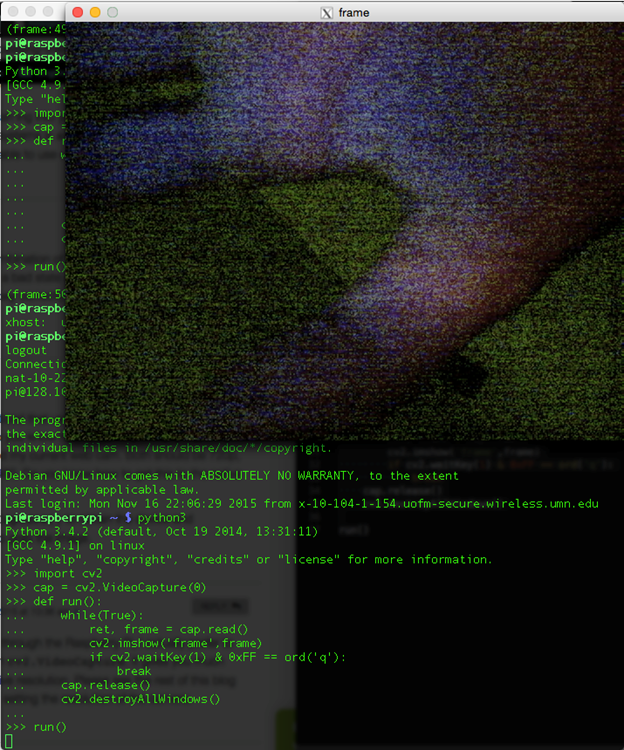
\includegraphics[height=9cm, width=7.5cm]{PS3_EYE}%
\label{fig_1}}
\caption{Example of PS3Eye Camera output connected to Raspberry Pi 2.}
\label{PS3_EYE}
\end{figure}

Also, through the use of the PS3Eye, the computer vision software, OpenCV \cite{opencv}, that was decided to be used was also experimented with to check compatibility on both the Raspberry Pi 2 Model B+ and the PS3Eye Camera, which also is displayed through Fig. \ref{PS3_EYE}.  Since the Air-Hockey Robot will need to detect an object and compute trajectory, the object recognition was experimented with as well. OpenCV’s built in feature detection software works on detecting features coming from the camera. However, the Basic SIFT feature detection is rather slow and error prone, even in C++. An example of this can be seen in Fig. \ref{OBJ_REC}, where the applications of SIFT was experimented with.  As mentioned in \ref{relatedwork}, if SIFT continually proves to be too slow moving forward, other algorithms for image processing can be used an order to decrease time-complexity.  Other methods of feature detection may need to be attempted or further experimentation of SIFT with a lower resolution of camera input will need to be examined and compared. This project decidedly does not need a high degree of resolution for detection of the puck, so this remains a viable option still.


\begin{figure}[!h]
\centering
\subfloat{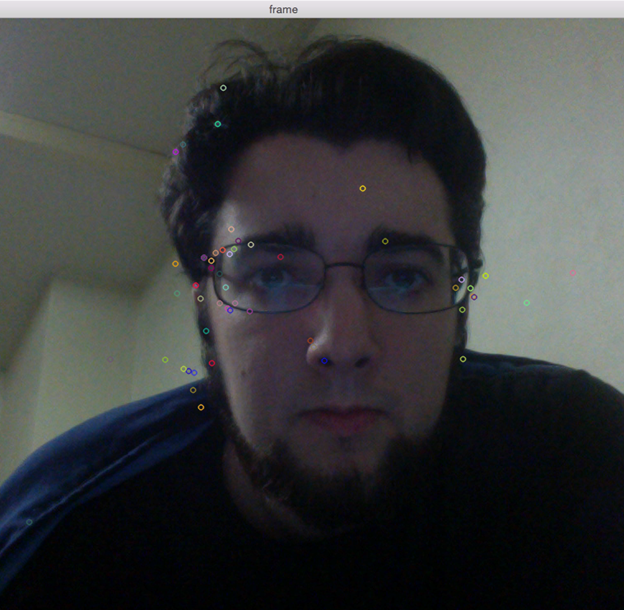
\includegraphics[height=8cm, width=8cm]{OBJ_REC}%
\label{fig_2}}
\caption{Example of OpenCV3 built in SIFT feature matching.}
\label{OBJ_REC}
\end{figure}


The ability to interface the Servo Motors, seen in Fig. \ref{servo}, with the Raspberry Pi 2 has also been explored.  The Raspberry Pi 2 has physical pins to which the Servo Motors can be attached and controlled through.  The Servo Motor can be connected to a breadboard, which in turn will be connected to certain pins on the Raspberry Pi 2.  The interface for the pins can be seen Fig. \ref{PIN_RP2}, which gives the necessary information for their use. The libraries necessary for making use of the Raspberry Pi Model B+ GPIO (General-purpose input/output) pins accessible have been installed onto the Raspberry Pi 2, but further testing needs to be done an order to assess it's full capability. The servo motors will also be able to be interfaced through the ROS, which provides a library for Servo Motor controls.  Through the use of this library, development time necessary will hopefully be decreased by a large degree of magnitude.

\begin{figure}[!h]
\centering
\subfloat{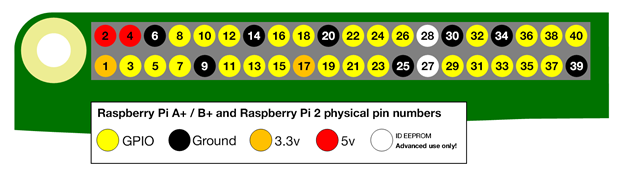
\includegraphics[height=3cm, width=9cm]{PIN_RP2}%
\label{fig_3}}
\caption{Raspberry Pi 2 GPIO pin numbers.}
\label{PIN_RP2}
\end{figure}


The Artificial Intelligence algorithms have been evaluated to a certain degree as well. The algorithms have been narrowed to those which can be performed in Real-Time and that involve a heuristic. The algorithms also need to be computationally light due to the time-complexity needed for the image processing with the computer vision.  With a real-time AI algorithm, a time constraint is placed on the algorithm such that the best path at the moment is taken without needing to fully evaluate the move.

\begin{figure}[!h]
\centering
\subfloat{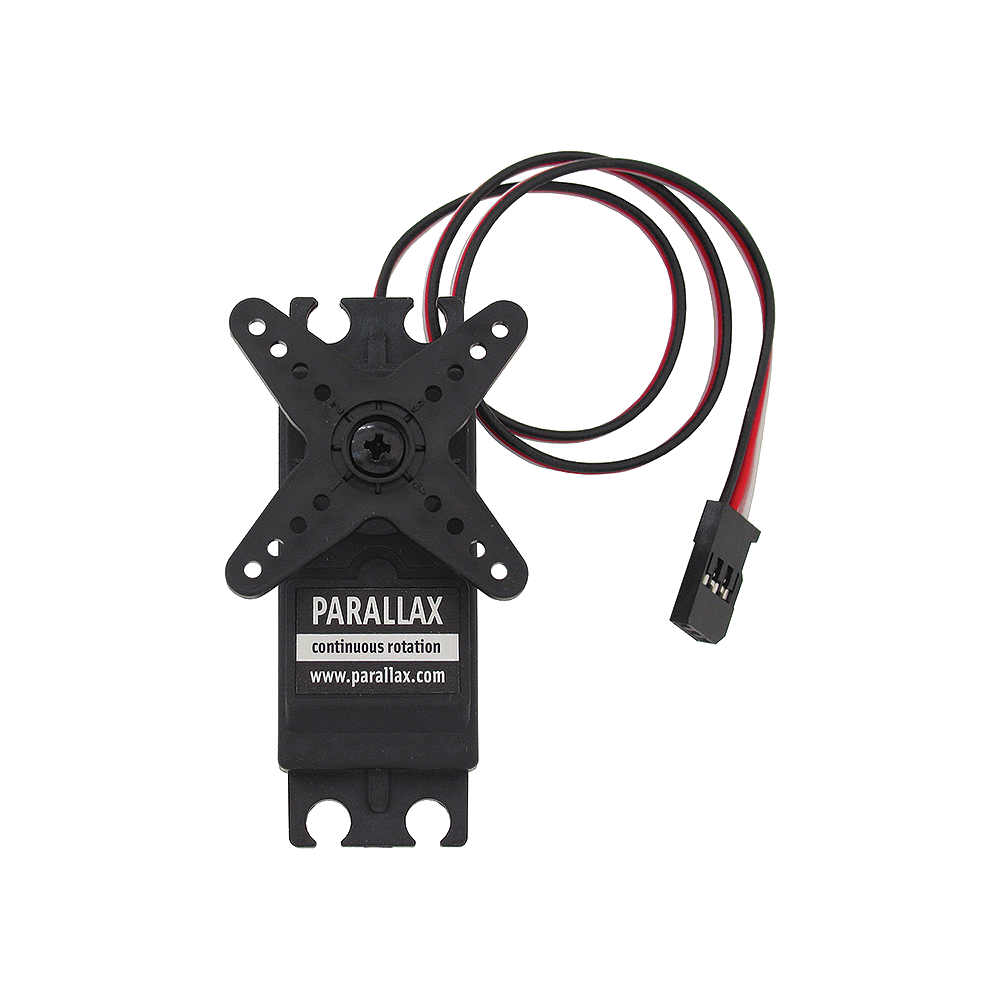
\includegraphics[height=9cm, width=9cm]{servo}%
\label{fig_5}}
\caption{Parallax Continuous Rotation Servo Motor.}
\label{servo}
\end{figure}

\subsection{Complications}

Some complications have been run into thus far in the project.  This section will further discuss the complications that were experienced and the reaction made due to them.  

One of the complications came with the Raspberry Pi 2 Model B+ and the desired operating system that was to be put onto it.  The original operating system that was going to put onto the Raspberry Pi 2 Model B+ was Arch-Linux due to how lightweight the operating system was.  Due to compatibility issues, Raspbian was placed as the software for it's ease of use.  Despite this complication, Raspbian will supply a better interface to work through which may speed up development time.  If development time can be sped up, then optimization can be explored sooner in the Air Hockey Playing Robot.  

Another complication that has been run into was the size of the servo motor connectors to the pulley belt wenches.  The solution this problem will consist of inserted a spaced between to the two to fill the gap and create a snug fit.  

Lastly, another complication was experienced with the fact that the Raspberry Pi 2 Model B+ only contained to five volt pins, which is a problem with a total of four servo motors.  This complication was addressed by adjusting the design slightly to include individual power supply for some/all of the motors.  This may be decidedly better than relying on the power from Raspberry Pi 2 board as well. 

All three complications experienced thus far have had rather quick reactionary fixes and none have been completely blocking to any degree.  As the project moves forward, it is expected that complications will only increase and will need to be dealt with as they come.  Since complications of this sort are unknown by their very nature, no predictive planning for possible complications will be set forth as it will only take away from implementation and construction time.  

\subsection{Future Timeline}
\begin{itemize}
\item Obtain Remaining Hardware 
\begin{itemize}
\item A few parts are still in route.  Of these are the remaining three servo motors, the belts for the motors, and a few other minor items.
\end{itemize}
\item Start Constructing Robot Manipulator onto the Air Hockey Table.
\item Start developing computer vision portions that will handle object recognition of a puck on the Air Hockey Table.
\begin{itemize}
\item This computer vision portion will be implemented through the OpenCV \cite{opencv} library.  This software will be used an order to speed up development as well as for feasibility reasons.
\end{itemize}
\item Start developing robotic manipulator controller software that provides an interface for controlling the servo motors in a coordinated fashion.
\begin{itemize}
\item The robotic manipulator controller software will make use of the ROS \cite{ros} library.  This will
\end{itemize}
\item Start creating transitional data-processing software layer
\begin{itemize}
\item This layer will be implemented within ROS portion of the software since the ROS provides a \textit{cv\_bridge} library which creates easy compatibility with preexisting OpenCV programs.
\item Develop Artificial Intelligence Algorithms that can be applied in a Real-time environment.
\begin{itemize}
\item The algorithms will first be developed defensively such that a puck can be blocked from entering the goal.  After this, the algorithms can start to be readjusted to account for offensive moves as well.  This will include not only entering the pace of the puck, but to strike to the puck back.  Lastly, the offensive algorithm will be further developed to account for striking the puck towards the goal in an effort to win.
\end{itemize}
\item Creating differing difficulty levels for A.I.
\end{itemize}
\item Experimentation and Data Collection
\begin{itemize}
\item The metrics discussed in \ref{introduction}. Introduction:
\begin{itemize}
\item Efficiency, which most likely be measured in distance.
\item Reactionary Time, which will most likely be measured the time it takes to go from image capture to robotic manipulator input.
\item Accuracy, which will most likely be measure as a percentage in which a puck was hit into the goal over all the times attempted.  This unit will most likely be displayed as a ratio between 0 and 1, which will allow for it to be plotted visibly on a relatively small y-scale.
\item Repeatability, which will most likely be measure through a computation that factors repetitious variance.  The equation used to measure this metric and the units will be investigated when implementation is complete and experimentation begins.
\end{itemize}
\item Tweaks to implementation
\begin{itemize}
\item As whether or not to use thresholding or shape matching for the computer vision portion.
\item The cost in reactionary time due to using a form of artificial intelligence instead of raw equations.  Also, the time-constraint (if given for the algorithm) decreasing/increasing based on experimental reactionary-time.
\end{itemize}
\end{itemize}
\item Analysis of the experimental data collected as well as of the project in it's entirety.
\item Final Report summarizing the process of building an Air Hockey Robot along with any valuable experimental data that was collected.
\end{itemize}
%%%%%%%%%%%%%%%%%%%%%%%%%%%%%%%%%%%%%%%%%%%%%%%%%%%%%%%%%%%%%%%%%%%%%%%%%%%%%%%%
\bibliographystyle{IEEEtran}
\bibliography{IEEEabrv,project}
\end{document}
